% Template for ICASSP-2021 paper; to be used with:
%          spconf.sty  - ICASSP/ICIP LaTeX style file, and
%          IEEEbib.bst - IEEE bibliography style file.
% --------------------------------------------------------------------------
\documentclass{article}
\usepackage{spconf,amsmath,graphicx}

% Example definitions.
% --------------------
\def\x{{\mathbf x}}
\def\L{{\cal L}}

% Title.
% ------
\title{Real-Time Audio Filtering}
%
% Single address.
% ---------------
\name{Rahul Choudhary}
\address{EE, IIT Kanpur}
%
\begin{document}
%
\maketitle
%
\begin{abstract}
This is a report for a course project named "Real-time Audio Filtering". The project is based on simple online audio processing techniques. I made a GUI using Tkinter in Python that is used to design filters. It takes input from microphone and gives output to speaker in real time. The user can specify which type of audio filter to apply on the input voice. The user can plot the characteristics (i.e. impulse response, magnitude response, phase response, and pole-zero plot) of the designed filter. Users are also able to see the plot of input sound and output sound along with their Frequency domain response in real time in a separate window.
\end{abstract}
%
\begin{keywords}
Introduction, The GUI, Filters, Plotting the filter characteristics, Real time Streaming
\end{keywords}
%
\section{Introduction}
\label{sec:intro}
I will be describing my project in the following sections along with an example on using the GUI to filter the audio in real time.
This GUI uses the input from the user to design the requested filter. The GUI is made using the {\bf tkinter} package in python. The filters are made using the {\bf scipy} library. The audio I/O is done using the {\bf PyAudio} that provides python binding for {\bf PortAudio}, the cross-platform audio I/O library.

\section{The GUI}
\label{sec:gui}

I made an interactive and dynamic GUI that asks user the preferences to design filter. It first asks the type of filter the user want to design, i.e. IIR of FIR. Then after selecting any one of these, we get a drop-down menu that ask for the input method the user want to give. It provides 3 options for IIR filter and 2 options for FIR filter. After selecting the desired method of input, the user is asked for the input values to design the filter. Once the values are set we can design the filter by clicking on the \emph{"Get filter response"} button.

To show an example, say we want a 3rd order lowpass IIR filter with cutoff frequency 1000 Hz. So first select IIR from the two options. Then select the input method as \emph{"Cutoff frequency (in Hz) and filter order"} as show in Fig.1(a). After this, select the \emph{lowpass} option from four options as \emph{lowpass, highpass, bandpass, and bandstop.}
Then the user will input the required cutoff frequency and filter order. Then simply click on \emph{"Set Values"} and then \emph{"Get Filter Response!"} buttons. See Fig.1(b). The filter is designed!
\begin{figure}[htb]

\begin{minipage}[b]{0.48\linewidth}
  \centering
  \centerline{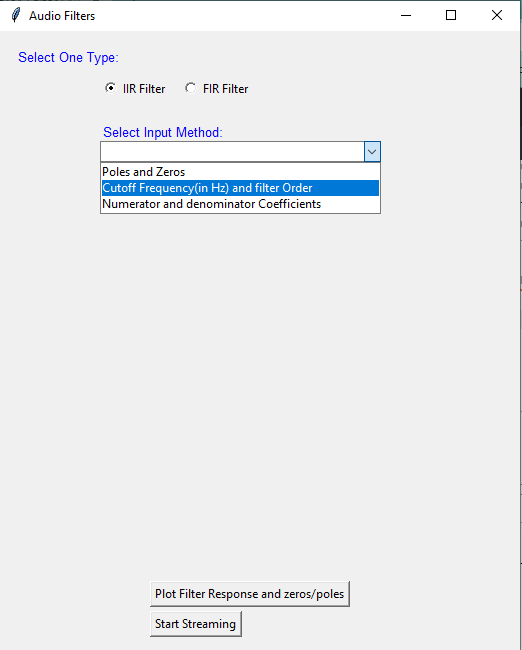
\includegraphics[width=4.2cm]{1}}
%  \vspace{2.0cm}
  \centerline{(a)}\medskip
\end{minipage}
%
\hfill
\begin{minipage}[b]{0.48\linewidth}
  \centering
  \centerline{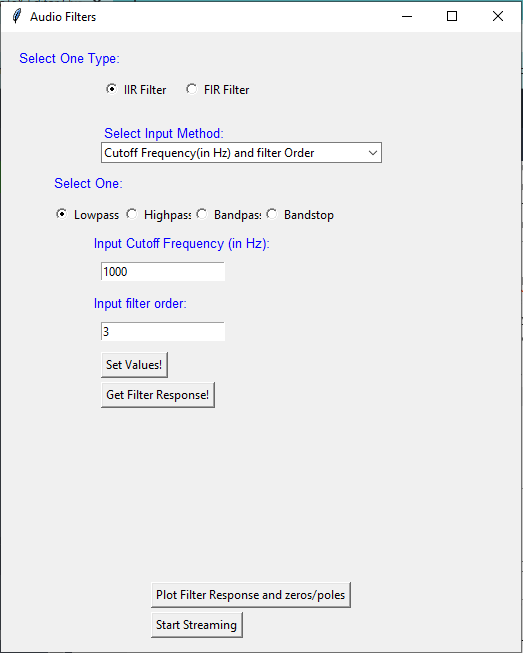
\includegraphics[width=4.2cm]{2}}
%  \vspace{1.5cm}
  \centerline{(b)}\medskip
\end{minipage}
%
\caption{}
\label{fig:fig1}
%
\end{figure}


\section{Filters}
\label{sec:filters}
The filters are designed based on the user input using\\
$scipy.signal$ module. For filters, I used \\$scipy.signal.freqz()$ or $scipy.signal.freq_zpk()$ function to get the filter response. The output of these functions is in the form ({\bf H, w}) where {\bf H} is the frequency response of the filter and {\bf w} contains the corresponding frequencies (in rad/s). After that it convert the frequency response to impulse response by simply taking the Inverse FFT of {\bf H}. It also calculate the zeros and poles and phase/magnitude response, for plotting purpose, while calculating the filter response. 

\section{Plotting the filter Characteristics}
\label{sec:plotting}
After we have designed our desired filter, we can also plot the filter characteristics to visualize our filter response. The plotting can simply be done by clicking the \emph{"Plot Filter Response and zeros/poles"} button on the GUI. It plot the Filter impulse response, Phase response, Magnitude response, and Poles and Zeros in a separate window.

The plot generated for our designed example filter is shown in Fig.2.

\begin{figure}[htb]
\centering
  \centerline{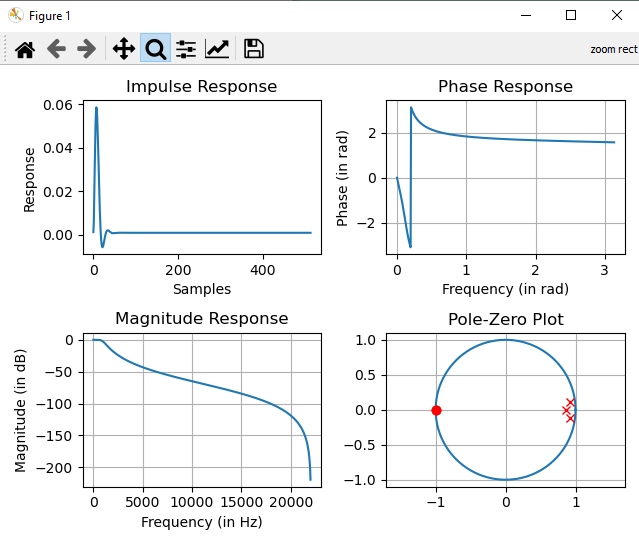
\includegraphics[width=8.5cm]{3}}
\caption{}
\label{fig:fig2}
\end{figure}


\section{Real time Streaming}
\label{sec:stream}
This is the part where the actual filtering of our voice is done. Once we are satisfied with the filter characteristics, we can move to real time filtering and streaming of our own voice. The input/output part of the process is done using the PyAudio python bindings for PortAudio. It takes input from our microphone, convert the signal to bytes. After this, we convert the data extracted to integer numpy array for further processing. We then have the input signal and the filter impulse response. We get the filtered signal simply by convolving the two signals. Now we have the input signal and the output signal. We calculate their FFTs for visualization purpose.

We plot the input and output signals along with their FFTs in a separate window so that we can visualize the frequencies of our voice and what is the response of the applied filter on our voice. An instance of this is shown in Fig.3. It shows that our lowpass filter is suppressing the high frequency noise.

\begin{figure}[htb]
\centering
  \centerline{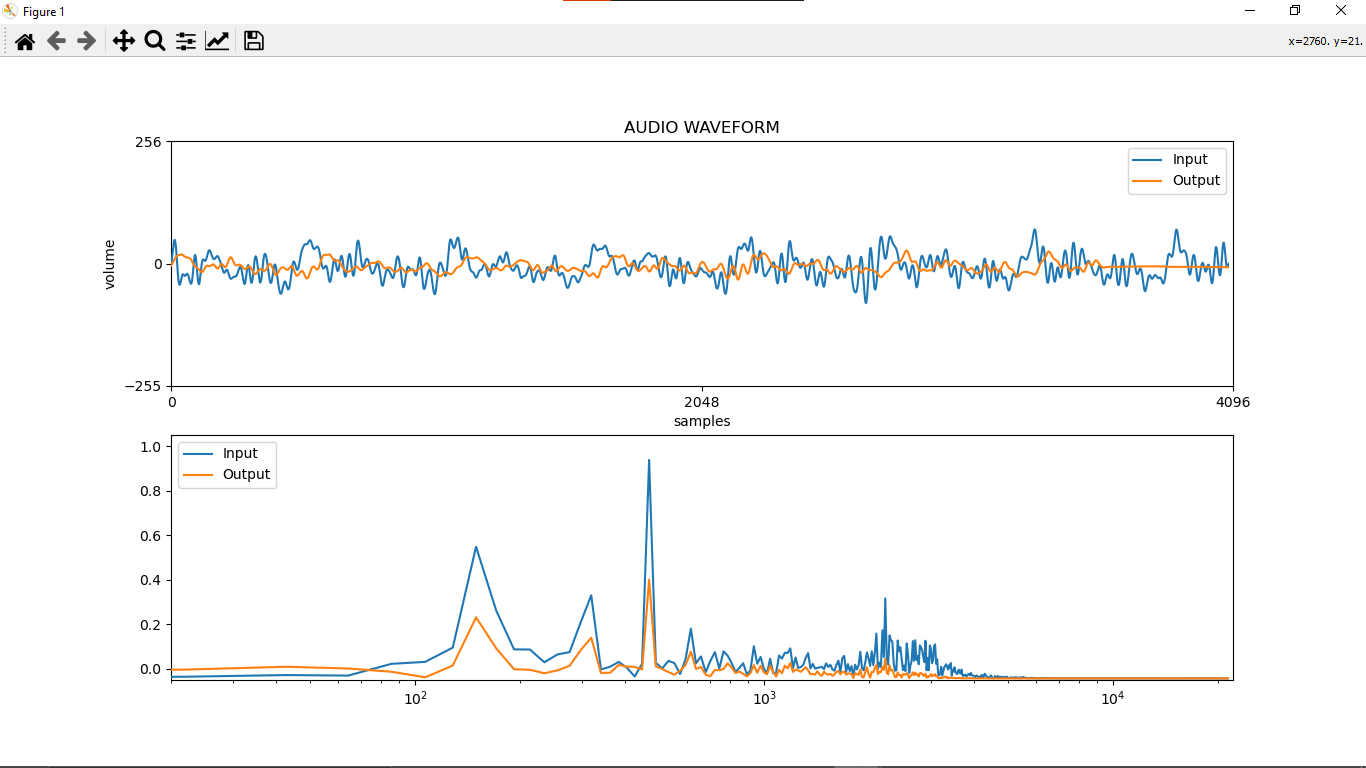
\includegraphics[width=8.5cm]{4}}
\caption{}
\label{fig:fig3}
\end{figure}


\section{REFERENCES}
\label{sec:refs}

1. EE301 (Digital Signal Processing) lectures, Dr. Vipul Arora\\
2. Stackoverflow (https://stackoverflow.com/)\\
3. Scipy open source Python library (https://www.scipy.org/)\\
4. Tkinter Python binding to Tk GUI toolkit\\ (https://docs.python.org/3/library/tkinter.html)\\
5. PyAudio python binding to PortAudio\\
(https://people.csail.mit.edu/hubert/pyaudio/)


\end{document}
